\documentclass[1p]{elsarticle_modified}
%\bibliographystyle{elsarticle-num}

%\usepackage[colorlinks]{hyperref}
%\usepackage{abbrmath_seonhwa} %\Abb, \Ascr, \Acal ,\Abf, \Afrak
\usepackage{amsfonts}
\usepackage{amssymb}
\usepackage{amsmath}
\usepackage{amsthm}
\usepackage{scalefnt}
\usepackage{amsbsy}
\usepackage{kotex}
\usepackage{caption}
\usepackage{subfig}
\usepackage{color}
\usepackage{graphicx}
\usepackage{xcolor} %% white, black, red, green, blue, cyan, magenta, yellow
\usepackage{float}
\usepackage{setspace}
\usepackage{hyperref}

\usepackage{tikz}
\usetikzlibrary{arrows}

\usepackage{multirow}
\usepackage{array} % fixed length table
\usepackage{hhline}

%%%%%%%%%%%%%%%%%%%%%
\makeatletter
\renewcommand*\env@matrix[1][\arraystretch]{%
	\edef\arraystretch{#1}%
	\hskip -\arraycolsep
	\let\@ifnextchar\new@ifnextchar
	\array{*\c@MaxMatrixCols c}}
\makeatother %https://tex.stackexchange.com/questions/14071/how-can-i-increase-the-line-spacing-in-a-matrix
%%%%%%%%%%%%%%%

\usepackage[normalem]{ulem}

\newcommand{\msout}[1]{\ifmmode\text{\sout{\ensuremath{#1}}}\else\sout{#1}\fi}
%SOURCE: \msout is \stkout macro in https://tex.stackexchange.com/questions/20609/strikeout-in-math-mode

\newcommand{\cancel}[1]{
	\ifmmode
	{\color{red}\msout{#1}}
	\else
	{\color{red}\sout{#1}}
	\fi
}

\newcommand{\add}[1]{
	{\color{blue}\uwave{#1}}
}

\newcommand{\replace}[2]{
	\ifmmode
	{\color{red}\msout{#1}}{\color{blue}\uwave{#2}}
	\else
	{\color{red}\sout{#1}}{\color{blue}\uwave{#2}}
	\fi
}

\newcommand{\Sol}{\mathcal{S}} %segment
\newcommand{\D}{D} %diagram
\newcommand{\A}{\mathcal{A}} %arc


%%%%%%%%%%%%%%%%%%%%%%%%%%%%%5 test

\def\sl{\operatorname{\textup{SL}}(2,\Cbb)}
\def\psl{\operatorname{\textup{PSL}}(2,\Cbb)}
\def\quan{\mkern 1mu \triangleright \mkern 1mu}

\theoremstyle{definition}
\newtheorem{thm}{Theorem}[section]
\newtheorem{prop}[thm]{Proposition}
\newtheorem{lem}[thm]{Lemma}
\newtheorem{ques}[thm]{Question}
\newtheorem{cor}[thm]{Corollary}
\newtheorem{defn}[thm]{Definition}
\newtheorem{exam}[thm]{Example}
\newtheorem{rmk}[thm]{Remark}
\newtheorem{alg}[thm]{Algorithm}

\newcommand{\I}{\sqrt{-1}}
\begin{document}

%\begin{frontmatter}
%
%\title{Boundary parabolic representations of knots up to 8 crossings}
%
%%% Group authors per affiliation:
%\author{Yunhi Cho} 
%\address{Department of Mathematics, University of Seoul, Seoul, Korea}
%\ead{yhcho@uos.ac.kr}
%
%
%\author{Seonhwa Kim} %\fnref{s_kim}}
%\address{Center for Geometry and Physics, Institute for Basic Science, Pohang, 37673, Korea}
%\ead{ryeona17@ibs.re.kr}
%
%\author{Hyuk Kim}
%\address{Department of Mathematical Sciences, Seoul National University, Seoul 08826, Korea}
%\ead{hyukkim@snu.ac.kr}
%
%\author{Seokbeom Yoon}
%\address{Department of Mathematical Sciences, Seoul National University, Seoul, 08826,  Korea}
%\ead{sbyoon15@snu.ac.kr}
%
%\begin{abstract}
%We find all boundary parabolic representation of knots up to 8 crossings.
%
%\end{abstract}
%\begin{keyword}
%    \MSC[2010] 57M25 
%\end{keyword}
%
%\end{frontmatter}

%\linenumbers
%\tableofcontents
%
\newcommand\colored[1]{\textcolor{white}{\rule[-0.35ex]{0.8em}{1.4ex}}\kern-0.8em\color{red} #1}%
%\newcommand\colored[1]{\textcolor{white}{ #1}\kern-2.17ex	\textcolor{white}{ #1}\kern-1.81ex	\textcolor{white}{ #1}\kern-2.15ex\color{red}#1	}

{\Large $\underline{12n_{0055}~(K12n_{0055})}$}

\setlength{\tabcolsep}{10pt}
\renewcommand{\arraystretch}{1.6}
\vspace{1cm}\begin{tabular}{m{100pt}>{\centering\arraybackslash}m{274pt}}
\multirow{5}{120pt}{
	\centering
	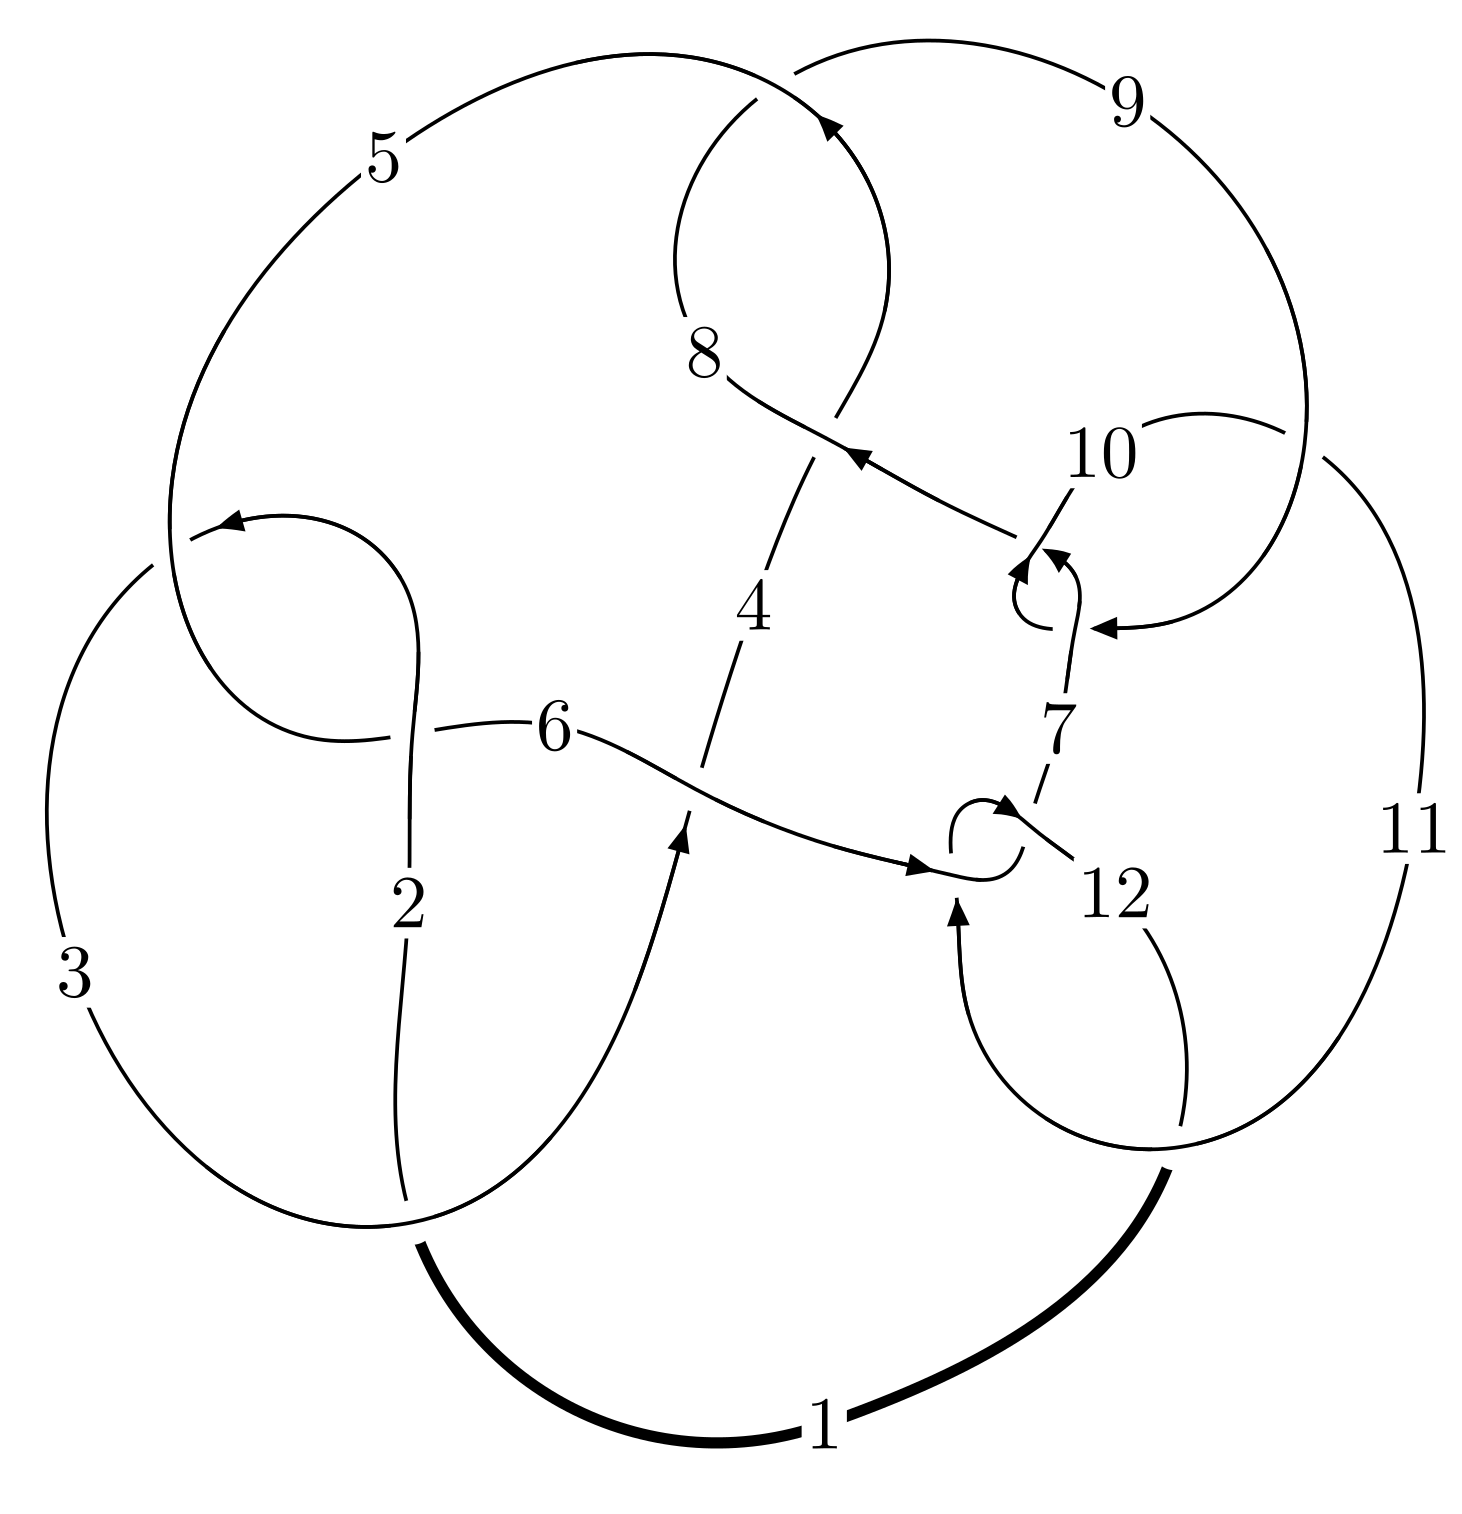
\includegraphics[width=112pt]{../../../GIT/diagram.site/Diagrams/png/2144_12n_0055.png}\\
\ \ \ A knot diagram\footnotemark}&
\allowdisplaybreaks
\textbf{Linearized knot diagam} \\
\cline{2-2}
 &
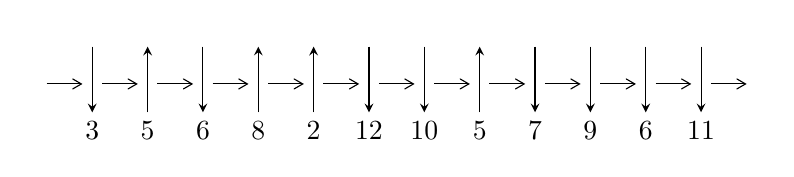
\begin{tikzpicture}[x=20pt, y=17pt]
	% nodes
	\node (C0) at (0, 0) {};
	\node (C1) at (1, 0) {};
	\node (C1U) at (1, +1) {};
	\node (C1D) at (1, -1) {3};

	\node (C2) at (2, 0) {};
	\node (C2U) at (2, +1) {};
	\node (C2D) at (2, -1) {5};

	\node (C3) at (3, 0) {};
	\node (C3U) at (3, +1) {};
	\node (C3D) at (3, -1) {6};

	\node (C4) at (4, 0) {};
	\node (C4U) at (4, +1) {};
	\node (C4D) at (4, -1) {8};

	\node (C5) at (5, 0) {};
	\node (C5U) at (5, +1) {};
	\node (C5D) at (5, -1) {2};

	\node (C6) at (6, 0) {};
	\node (C6U) at (6, +1) {};
	\node (C6D) at (6, -1) {12};

	\node (C7) at (7, 0) {};
	\node (C7U) at (7, +1) {};
	\node (C7D) at (7, -1) {10};

	\node (C8) at (8, 0) {};
	\node (C8U) at (8, +1) {};
	\node (C8D) at (8, -1) {5};

	\node (C9) at (9, 0) {};
	\node (C9U) at (9, +1) {};
	\node (C9D) at (9, -1) {7};

	\node (C10) at (10, 0) {};
	\node (C10U) at (10, +1) {};
	\node (C10D) at (10, -1) {9};

	\node (C11) at (11, 0) {};
	\node (C11U) at (11, +1) {};
	\node (C11D) at (11, -1) {6};

	\node (C12) at (12, 0) {};
	\node (C12U) at (12, +1) {};
	\node (C12D) at (12, -1) {11};
	\node (C13) at (13, 0) {};

	% arrows
	\draw[->,>={angle 60}]
	(C0) edge (C1) (C1) edge (C2) (C2) edge (C3) (C3) edge (C4) (C4) edge (C5) (C5) edge (C6) (C6) edge (C7) (C7) edge (C8) (C8) edge (C9) (C9) edge (C10) (C10) edge (C11) (C11) edge (C12) (C12) edge (C13) ;	\draw[->,>=stealth]
	(C1U) edge (C1D) (C2D) edge (C2U) (C3U) edge (C3D) (C4D) edge (C4U) (C5D) edge (C5U) (C6U) edge (C6D) (C7U) edge (C7D) (C8D) edge (C8U) (C9U) edge (C9D) (C10U) edge (C10D) (C11U) edge (C11D) (C12U) edge (C12D) ;
	\end{tikzpicture} \\
\hhline{~~} \\& 
\textbf{Solving Sequence} \\ \cline{2-2} 
 &
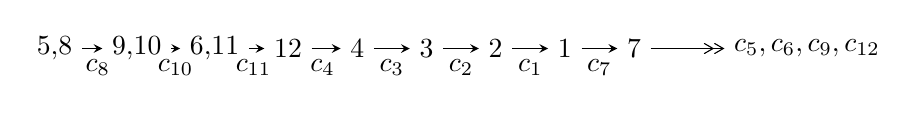
\begin{tikzpicture}[x=25pt, y=7pt]
	% node
	\node (A0) at (-1/8, 0) {5,8};
	\node (A1) at (17/16, 0) {9,10};
	\node (A2) at (35/16, 0) {6,11};
	\node (A3) at (13/4, 0) {12};
	\node (A4) at (17/4, 0) {4};
	\node (A5) at (21/4, 0) {3};
	\node (A6) at (25/4, 0) {2};
	\node (A7) at (29/4, 0) {1};
	\node (A8) at (33/4, 0) {7};
	\node (C1) at (1/2, -1) {$c_{8}$};
	\node (C2) at (13/8, -1) {$c_{10}$};
	\node (C3) at (11/4, -1) {$c_{11}$};
	\node (C4) at (15/4, -1) {$c_{4}$};
	\node (C5) at (19/4, -1) {$c_{3}$};
	\node (C6) at (23/4, -1) {$c_{2}$};
	\node (C7) at (27/4, -1) {$c_{1}$};
	\node (C8) at (31/4, -1) {$c_{7}$};
	\node (A9) at (43/4, 0) {$c_{5},c_{6},c_{9},c_{12}$};

	% edge
	\draw[->,>=stealth]	
	(A0) edge (A1) (A1) edge (A2) (A2) edge (A3) (A3) edge (A4) (A4) edge (A5) (A5) edge (A6) (A6) edge (A7) (A7) edge (A8) ;
	\draw[->>,>={angle 60}]	
	(A8) edge (A9);
\end{tikzpicture} \\ 

\end{tabular} \\

\footnotetext{
The image of knot diagram is generated by the software ``\textbf{Draw programme}" developed by Andrew Bartholomew(\url{http://www.layer8.co.uk/maths/draw/index.htm\#Running-draw}), where we modified some parts for our purpose(\url{https://github.com/CATsTAILs/LinksPainter}).
}\phantom \\ \newline 
\centering \textbf{Ideals for irreducible components\footnotemark of $X_{\text{par}}$} 
 
\begin{align*}
I^u_{1}&=\langle 
-1.43951\times10^{32} u^{27}+3.79444\times10^{32} u^{26}+\cdots+9.42397\times10^{33} d+5.95648\times10^{32},\\
\phantom{I^u_{1}}&\phantom{= \langle  }5.68907\times10^{31} u^{27}-1.81131\times10^{32} u^{26}+\cdots+1.88479\times10^{34} c-1.63326\times10^{34},\\
\phantom{I^u_{1}}&\phantom{= \langle  }7.06990\times10^{32} u^{27}-2.19194\times10^{33} u^{26}+\cdots+9.42397\times10^{33} b-2.89436\times10^{34},\\
\phantom{I^u_{1}}&\phantom{= \langle  }-6.86736\times10^{32} u^{27}+2.01828\times10^{33} u^{26}+\cdots+1.88479\times10^{34} a+1.76377\times10^{34},\\
\phantom{I^u_{1}}&\phantom{= \langle  }u^{28}-3 u^{27}+\cdots-64 u+32\rangle \\
I^u_{2}&=\langle 
-4182326921 u^{19} c-3076005459 u^{19}+\cdots+29433713862 c-28068851486,\\
\phantom{I^u_{2}}&\phantom{= \langle  }49133842327 u^{19} c-33157787379 u^{19}+\cdots-204672432210 c+75288972938,\\
\phantom{I^u_{2}}&\phantom{= \langle  }-96297864 u^{19}+56397459 u^{18}+\cdots+6762765143 b+683924131,\\
\phantom{I^u_{2}}&\phantom{= \langle  }4877710595 u^{19}+3159804985 u^{18}+\cdots+108204242288 a+50023322678,\\
\phantom{I^u_{2}}&\phantom{= \langle  }u^{20}+u^{19}+\cdots-8 u-4\rangle \\
\\
I^v_{1}&=\langle 
a,\;d,\;c-1,\;b+1,\;v^2+v+1\rangle \\
I^v_{2}&=\langle 
a,\;d-1,\;c+a-1,\;b+1,\;v^2+v+1\rangle \\
I^v_{3}&=\langle 
c,\;d-1,\;b,\;a+1,\;v+1\rangle \\
I^v_{4}&=\langle 
c,\;d-1,\;v^2 b a+v^2 b- a v+c- v-1,\;b^2 v^2- b v+1\rangle \\
\end{align*}
\raggedright * 5 irreducible components of $\dim_{\mathbb{C}}=0$, with total 73 representations.\\
\raggedright * 1 irreducible components of $\dim_{\mathbb{C}}=1$ \\
\footnotetext{All coefficients of polynomials are rational numbers. But the coefficients are sometimes approximated in decimal forms when there is not enough margin.}
\newpage
\renewcommand{\arraystretch}{1}
\centering \section*{I. $I^u_{1}= \langle -1.44\times10^{32} u^{27}+3.79\times10^{32} u^{26}+\cdots+9.42\times10^{33} d+5.96\times10^{32},\;5.69\times10^{31} u^{27}-1.81\times10^{32} u^{26}+\cdots+1.88\times10^{34} c-1.63\times10^{34},\;7.07\times10^{32} u^{27}-2.19\times10^{33} u^{26}+\cdots+9.42\times10^{33} b-2.89\times10^{34},\;-6.87\times10^{32} u^{27}+2.02\times10^{33} u^{26}+\cdots+1.88\times10^{34} a+1.76\times10^{34},\;u^{28}-3 u^{27}+\cdots-64 u+32 \rangle$}
\flushleft \textbf{(i) Arc colorings}\\
\begin{tabular}{m{7pt} m{180pt} m{7pt} m{180pt} }
\flushright $a_{5}=$&$\begin{pmatrix}0\\u\end{pmatrix}$ \\
\flushright $a_{8}=$&$\begin{pmatrix}1\\0\end{pmatrix}$ \\
\flushright $a_{9}=$&$\begin{pmatrix}1\\- u^2\end{pmatrix}$ \\
\flushright $a_{10}=$&$\begin{pmatrix}-0.00301840 u^{27}+0.00961014 u^{26}+\cdots-0.512168 u+0.866547\\0.0152750 u^{27}-0.0402637 u^{26}+\cdots+1.56827 u-0.0632056\end{pmatrix}$ \\
\flushright $a_{6}=$&$\begin{pmatrix}0.0364356 u^{27}-0.107082 u^{26}+\cdots+4.89194 u-0.935790\\-0.0750204 u^{27}+0.232591 u^{26}+\cdots-10.9778 u+3.07128\end{pmatrix}$ \\
\flushright $a_{11}=$&$\begin{pmatrix}-0.0188045 u^{27}+0.0531544 u^{26}+\cdots-2.21254 u+0.947510\\0.00903337 u^{27}-0.0298398 u^{26}+\cdots+1.30721 u-0.185253\end{pmatrix}$ \\
\flushright $a_{12}=$&$\begin{pmatrix}-0.0414237 u^{27}+0.136562 u^{26}+\cdots-6.59726 u+2.19775\\0.0656027 u^{27}-0.212991 u^{26}+\cdots+10.4331 u-2.93689\end{pmatrix}$ \\
\flushright $a_{4}=$&$\begin{pmatrix}- u\\u\end{pmatrix}$ \\
\flushright $a_{3}=$&$\begin{pmatrix}0.0439376 u^{27}-0.115337 u^{26}+\cdots+2.49821 u+0.486668\\-0.0676735 u^{27}+0.181595 u^{26}+\cdots-5.26458 u-0.607411\end{pmatrix}$ \\
\flushright $a_{2}=$&$\begin{pmatrix}0.0439376 u^{27}-0.115337 u^{26}+\cdots+2.49821 u+0.486668\\-0.0724643 u^{27}+0.187953 u^{26}+\cdots-5.61617 u-1.13462\end{pmatrix}$ \\
\flushright $a_{1}=$&$\begin{pmatrix}0.0385848 u^{27}-0.125509 u^{26}+\cdots+6.08587 u-2.13549\\-0.0540378 u^{27}+0.180613 u^{26}+\cdots-9.11878 u+2.75912\end{pmatrix}$ \\
\flushright $a_{7}=$&$\begin{pmatrix}-0.00301840 u^{27}+0.00961014 u^{26}+\cdots-0.512168 u+0.866547\\-0.0157861 u^{27}+0.0435442 u^{26}+\cdots-1.70037 u+0.0809635\end{pmatrix}$\\&\end{tabular}
\flushleft \textbf{(ii) Obstruction class $= -1$}\\~\\
\flushleft \textbf{(iii) Cusp Shapes $= -0.217306 u^{27}+0.532528 u^{26}+\cdots-20.8205 u-2.69421$}\\~\\
\newpage\renewcommand{\arraystretch}{1}
\flushleft \textbf{(iv) u-Polynomials at the component}\newline \\
\begin{tabular}{m{50pt}|m{274pt}}
Crossings & \hspace{64pt}u-Polynomials at each crossing \\
\hline $$\begin{aligned}c_{1}\end{aligned}$$&$\begin{aligned}
&u^{28}+9 u^{27}+\cdots-56 u+16
\end{aligned}$\\
\hline $$\begin{aligned}c_{2},c_{5}\end{aligned}$$&$\begin{aligned}
&u^{28}+u^{27}+\cdots+8 u+4
\end{aligned}$\\
\hline $$\begin{aligned}c_{3}\end{aligned}$$&$\begin{aligned}
&u^{28}- u^{27}+\cdots+1736 u+1252
\end{aligned}$\\
\hline $$\begin{aligned}c_{4},c_{8}\end{aligned}$$&$\begin{aligned}
&u^{28}-3 u^{27}+\cdots-64 u+32
\end{aligned}$\\
\hline $$\begin{aligned}c_{6},c_{7},c_{9}\\c_{11}\end{aligned}$$&$\begin{aligned}
&u^{28}-5 u^{27}+\cdots-3 u+1
\end{aligned}$\\
\hline $$\begin{aligned}c_{10},c_{12}\end{aligned}$$&$\begin{aligned}
&u^{28}+9 u^{27}+\cdots+u+1
\end{aligned}$\\
\hline
\end{tabular}\\~\\
\newpage\renewcommand{\arraystretch}{1}
\flushleft \textbf{(v) Riley Polynomials at the component}\newline \\
\begin{tabular}{m{50pt}|m{274pt}}
Crossings & \hspace{64pt}Riley Polynomials at each crossing \\
\hline $$\begin{aligned}c_{1}\end{aligned}$$&$\begin{aligned}
&y^{28}+21 y^{27}+\cdots-6432 y+256
\end{aligned}$\\
\hline $$\begin{aligned}c_{2},c_{5}\end{aligned}$$&$\begin{aligned}
&y^{28}+9 y^{27}+\cdots-56 y+16
\end{aligned}$\\
\hline $$\begin{aligned}c_{3}\end{aligned}$$&$\begin{aligned}
&y^{28}+33 y^{27}+\cdots-17874936 y+1567504
\end{aligned}$\\
\hline $$\begin{aligned}c_{4},c_{8}\end{aligned}$$&$\begin{aligned}
&y^{28}-15 y^{27}+\cdots+3072 y+1024
\end{aligned}$\\
\hline $$\begin{aligned}c_{6},c_{7},c_{9}\\c_{11}\end{aligned}$$&$\begin{aligned}
&y^{28}-9 y^{27}+\cdots- y+1
\end{aligned}$\\
\hline $$\begin{aligned}c_{10},c_{12}\end{aligned}$$&$\begin{aligned}
&y^{28}+31 y^{27}+\cdots+39 y+1
\end{aligned}$\\
\hline
\end{tabular}\\~\\
\newpage\flushleft \textbf{(vi) Complex Volumes and Cusp Shapes}
$$\begin{array}{c|c|c}  
\text{Solutions to }I^u_{1}& \I (\text{vol} + \sqrt{-1}CS) & \text{Cusp shape}\\
 \hline 
\begin{aligned}
u &= \phantom{-}0.387721 + 0.851263 I \\
a &= -0.858816 + 0.725565 I \\
b &= \phantom{-}1.19972 - 1.08591 I \\
c &= \phantom{-}0.488405 - 0.103669 I \\
d &= \phantom{-}0.959210 + 0.415864 I\end{aligned}
 & -4.11180 - 3.97036 I & -11.03599 + 5.92521 I \\ \hline\begin{aligned}
u &= \phantom{-}0.387721 - 0.851263 I \\
a &= -0.858816 - 0.725565 I \\
b &= \phantom{-}1.19972 + 1.08591 I \\
c &= \phantom{-}0.488405 + 0.103669 I \\
d &= \phantom{-}0.959210 - 0.415864 I\end{aligned}
 & -4.11180 + 3.97036 I & -11.03599 - 5.92521 I \\ \hline\begin{aligned}
u &= -0.048850 + 0.802561 I \\
a &= \phantom{-}0.029080 - 0.305052 I \\
b &= -0.065828 + 1.072140 I \\
c &= \phantom{-}0.570907 + 0.125829 I \\
d &= \phantom{-}0.670453 - 0.368171 I\end{aligned}
 & -1.00554 + 1.45329 I & -3.70692 - 4.69342 I \\ \hline\begin{aligned}
u &= -0.048850 - 0.802561 I \\
a &= \phantom{-}0.029080 + 0.305052 I \\
b &= -0.065828 - 1.072140 I \\
c &= \phantom{-}0.570907 - 0.125829 I \\
d &= \phantom{-}0.670453 + 0.368171 I\end{aligned}
 & -1.00554 - 1.45329 I & -3.70692 + 4.69342 I \\ \hline\begin{aligned}
u &= \phantom{-}1.195800 + 0.230197 I \\
a &= -1.033490 - 0.671818 I \\
b &= -0.010332 + 0.550938 I \\
c &= \phantom{-}0.28063 - 1.44187 I \\
d &= -0.869944 + 0.668233 I\end{aligned}
 & \phantom{-}0.294538 + 1.243650 I & -3.92766 - 2.52803 I \\ \hline\begin{aligned}
u &= \phantom{-}1.195800 - 0.230197 I \\
a &= -1.033490 + 0.671818 I \\
b &= -0.010332 - 0.550938 I \\
c &= \phantom{-}0.28063 + 1.44187 I \\
d &= -0.869944 - 0.668233 I\end{aligned}
 & \phantom{-}0.294538 - 1.243650 I & -3.92766 + 2.52803 I\\
 \hline 
 \end{array}$$\newpage$$\begin{array}{c|c|c}  
\text{Solutions to }I^u_{1}& \I (\text{vol} + \sqrt{-1}CS) & \text{Cusp shape}\\
 \hline 
\begin{aligned}
u &= \phantom{-}0.512543 + 0.548760 I \\
a &= \phantom{-}0.511467 + 0.677219 I \\
b &= \phantom{-}0.399127 + 0.038680 I \\
c &= \phantom{-}0.810755 + 0.367303 I \\
d &= \phantom{-}0.023376 - 0.463629 I\end{aligned}
 & \phantom{-}0.77284 + 1.38296 I & \phantom{-}2.12358 - 4.20585 I \\ \hline\begin{aligned}
u &= \phantom{-}0.512543 - 0.548760 I \\
a &= \phantom{-}0.511467 - 0.677219 I \\
b &= \phantom{-}0.399127 - 0.038680 I \\
c &= \phantom{-}0.810755 - 0.367303 I \\
d &= \phantom{-}0.023376 + 0.463629 I\end{aligned}
 & \phantom{-}0.77284 - 1.38296 I & \phantom{-}2.12358 + 4.20585 I \\ \hline\begin{aligned}
u &= \phantom{-}1.240340 + 0.558685 I \\
a &= -0.781492 + 0.727914 I \\
b &= \phantom{-}0.253028 - 0.776710 I \\
c &= -0.19285 - 1.48947 I \\
d &= -1.085500 + 0.660311 I\end{aligned}
 & -1.36469 + 9.34331 I & -7.27750 - 7.90351 I \\ \hline\begin{aligned}
u &= \phantom{-}1.240340 - 0.558685 I \\
a &= -0.781492 - 0.727914 I \\
b &= \phantom{-}0.253028 + 0.776710 I \\
c &= -0.19285 + 1.48947 I \\
d &= -1.085500 - 0.660311 I\end{aligned}
 & -1.36469 - 9.34331 I & -7.27750 + 7.90351 I \\ \hline\begin{aligned}
u &= -0.306891 + 1.332240 I \\
a &= -0.939869 + 0.149572 I \\
b &= -0.419071 + 0.240287 I \\
c &= \phantom{-}0.448937 + 0.172706 I \\
d &= \phantom{-}0.940326 - 0.746445 I\end{aligned}
 & \phantom{-}2.80790 + 2.77377 I & -2.82329 - 2.35775 I \\ \hline\begin{aligned}
u &= -0.306891 - 1.332240 I \\
a &= -0.939869 - 0.149572 I \\
b &= -0.419071 - 0.240287 I \\
c &= \phantom{-}0.448937 - 0.172706 I \\
d &= \phantom{-}0.940326 + 0.746445 I\end{aligned}
 & \phantom{-}2.80790 - 2.77377 I & -2.82329 + 2.35775 I\\
 \hline 
 \end{array}$$\newpage$$\begin{array}{c|c|c}  
\text{Solutions to }I^u_{1}& \I (\text{vol} + \sqrt{-1}CS) & \text{Cusp shape}\\
 \hline 
\begin{aligned}
u &= -0.599185 + 0.160658 I \\
a &= \phantom{-}1.46524 - 1.11304 I \\
b &= -0.040138 + 0.305232 I \\
c &= \phantom{-}1.279080 - 0.454824 I \\
d &= -0.305944 + 0.246798 I\end{aligned}
 & -0.29820 + 2.58448 I & \phantom{-}1.60498 - 4.48843 I \\ \hline\begin{aligned}
u &= -0.599185 - 0.160658 I \\
a &= \phantom{-}1.46524 + 1.11304 I \\
b &= -0.040138 - 0.305232 I \\
c &= \phantom{-}1.279080 + 0.454824 I \\
d &= -0.305944 - 0.246798 I\end{aligned}
 & -0.29820 - 2.58448 I & \phantom{-}1.60498 + 4.48843 I \\ \hline\begin{aligned}
u &= \phantom{-}0.449039 + 1.329150 I \\
a &= -1.106900 - 0.095973 I \\
b &= -0.328030 + 0.364080 I \\
c &= \phantom{-}0.437109 - 0.156367 I \\
d &= \phantom{-}1.028210 + 0.725550 I\end{aligned}
 & \phantom{-}2.18074 - 8.77807 I & -4.21049 + 7.13120 I \\ \hline\begin{aligned}
u &= \phantom{-}0.449039 - 1.329150 I \\
a &= -1.106900 + 0.095973 I \\
b &= -0.328030 - 0.364080 I \\
c &= \phantom{-}0.437109 + 0.156367 I \\
d &= \phantom{-}1.028210 - 0.725550 I\end{aligned}
 & \phantom{-}2.18074 + 8.77807 I & -4.21049 - 7.13120 I \\ \hline\begin{aligned}
u &= -1.36520 + 0.37405 I \\
a &= -0.546646 + 0.073706 I \\
b &= -0.536551 + 0.044814 I \\
c &= \phantom{-}0.022772 + 1.320010 I \\
d &= -0.986935 - 0.757343 I\end{aligned}
 & \phantom{-}3.38586 - 5.92225 I & -1.05943 + 5.53498 I \\ \hline\begin{aligned}
u &= -1.36520 - 0.37405 I \\
a &= -0.546646 - 0.073706 I \\
b &= -0.536551 - 0.044814 I \\
c &= \phantom{-}0.022772 - 1.320010 I \\
d &= -0.986935 + 0.757343 I\end{aligned}
 & \phantom{-}3.38586 + 5.92225 I & -1.05943 - 5.53498 I\\
 \hline 
 \end{array}$$\newpage$$\begin{array}{c|c|c}  
\text{Solutions to }I^u_{1}& \I (\text{vol} + \sqrt{-1}CS) & \text{Cusp shape}\\
 \hline 
\begin{aligned}
u &= \phantom{-}0.128781 + 0.527754 I \\
a &= \phantom{-}1.29102 + 1.56415 I \\
b &= -2.31393 - 3.07959 I \\
c &= \phantom{-}0.536628 - 0.033094 I \\
d &= \phantom{-}0.856428 + 0.114486 I\end{aligned}
 & -2.91457 + 1.71407 I & -11.28016 - 2.34859 I \\ \hline\begin{aligned}
u &= \phantom{-}0.128781 - 0.527754 I \\
a &= \phantom{-}1.29102 - 1.56415 I \\
b &= -2.31393 + 3.07959 I \\
c &= \phantom{-}0.536628 + 0.033094 I \\
d &= \phantom{-}0.856428 - 0.114486 I\end{aligned}
 & -2.91457 - 1.71407 I & -11.28016 + 2.34859 I \\ \hline\begin{aligned}
u &= \phantom{-}1.36013 + 0.80195 I \\
a &= \phantom{-}0.214279 + 1.068830 I \\
b &= \phantom{-}0.00712 - 2.44927 I \\
c &= -0.423558 - 1.271240 I \\
d &= -1.23591 + 0.70803 I\end{aligned}
 & \phantom{-}5.1047 + 16.3284 I & -4.49305 - 9.50798 I \\ \hline\begin{aligned}
u &= \phantom{-}1.36013 - 0.80195 I \\
a &= \phantom{-}0.214279 - 1.068830 I \\
b &= \phantom{-}0.00712 + 2.44927 I \\
c &= -0.423558 + 1.271240 I \\
d &= -1.23591 - 0.70803 I\end{aligned}
 & \phantom{-}5.1047 - 16.3284 I & -4.49305 + 9.50798 I \\ \hline\begin{aligned}
u &= -1.41454 + 0.73498 I \\
a &= \phantom{-}0.133893 - 0.804174 I \\
b &= -0.47661 + 2.09588 I \\
c &= -0.342095 + 1.249650 I \\
d &= -1.20379 - 0.74444 I\end{aligned}
 & \phantom{-}6.34910 - 10.12380 I & -2.60535 + 5.05088 I \\ \hline\begin{aligned}
u &= -1.41454 - 0.73498 I \\
a &= \phantom{-}0.133893 + 0.804174 I \\
b &= -0.47661 - 2.09588 I \\
c &= -0.342095 - 1.249650 I \\
d &= -1.20379 + 0.74444 I\end{aligned}
 & \phantom{-}6.34910 + 10.12380 I & -2.60535 - 5.05088 I\\
 \hline 
 \end{array}$$\newpage$$\begin{array}{c|c|c}  
\text{Solutions to }I^u_{1}& \I (\text{vol} + \sqrt{-1}CS) & \text{Cusp shape}\\
 \hline 
\begin{aligned}
u &= \phantom{-}1.57578 + 0.34473 I \\
a &= \phantom{-}0.069527 + 1.019780 I \\
b &= \phantom{-}0.22695 - 2.42039 I \\
c &= \phantom{-}0.317772 + 0.829753 I \\
d &= -0.597487 - 1.051030 I\end{aligned}
 & \phantom{-}9.40632 + 3.24641 I & \phantom{-}0.187126 - 1.202849 I \\ \hline\begin{aligned}
u &= \phantom{-}1.57578 - 0.34473 I \\
a &= \phantom{-}0.069527 - 1.019780 I \\
b &= \phantom{-}0.22695 + 2.42039 I \\
c &= \phantom{-}0.317772 - 0.829753 I \\
d &= -0.597487 + 1.051030 I\end{aligned}
 & \phantom{-}9.40632 - 3.24641 I & \phantom{-}0.187126 + 1.202849 I \\ \hline\begin{aligned}
u &= -1.61547 + 0.19947 I \\
a &= \phantom{-}0.052706 - 0.927660 I \\
b &= -0.39545 + 2.29628 I \\
c &= \phantom{-}0.265518 - 0.890486 I \\
d &= -0.692497 + 1.031290 I\end{aligned}
 & \phantom{-}9.82407 + 3.16258 I & \phantom{-}0.50415 - 3.81889 I \\ \hline\begin{aligned}
u &= -1.61547 - 0.19947 I \\
a &= \phantom{-}0.052706 + 0.927660 I \\
b &= -0.39545 - 2.29628 I \\
c &= \phantom{-}0.265518 + 0.890486 I \\
d &= -0.692497 - 1.031290 I\end{aligned}
 & \phantom{-}9.82407 - 3.16258 I & \phantom{-}0.50415 + 3.81889 I\\
 \hline 
 \end{array}$$\newpage\newpage\renewcommand{\arraystretch}{1}
\centering \section*{II. $I^u_{2}= \langle -4.18\times10^{9} c u^{19}-3.08\times10^{9} u^{19}+\cdots+2.94\times10^{10} c-2.81\times10^{10},\;4.91\times10^{10} c u^{19}-3.32\times10^{10} u^{19}+\cdots-2.05\times10^{11} c+7.53\times10^{10},\;-9.63\times10^{7} u^{19}+5.64\times10^{7} u^{18}+\cdots+6.76\times10^{9} b+6.84\times10^{8},\;4.88\times10^{9} u^{19}+3.16\times10^{9} u^{18}+\cdots+1.08\times10^{11} a+5.00\times10^{10},\;u^{20}+u^{19}+\cdots-8 u-4 \rangle$}
\flushleft \textbf{(i) Arc colorings}\\
\begin{tabular}{m{7pt} m{180pt} m{7pt} m{180pt} }
\flushright $a_{5}=$&$\begin{pmatrix}0\\u\end{pmatrix}$ \\
\flushright $a_{8}=$&$\begin{pmatrix}1\\0\end{pmatrix}$ \\
\flushright $a_{9}=$&$\begin{pmatrix}1\\- u^2\end{pmatrix}$ \\
\flushright $a_{10}=$&$\begin{pmatrix}c\\0.154609 c u^{19}+0.113711 u^{19}+\cdots-1.08808 c+1.03762\end{pmatrix}$ \\
\flushright $a_{6}=$&$\begin{pmatrix}-0.0450787 u^{19}-0.0292022 u^{18}+\cdots-0.0198092 u-0.462305\\0.0142394 u^{19}-0.00833941 u^{18}+\cdots+0.752305 u-0.101131\end{pmatrix}$ \\
\flushright $a_{11}=$&$\begin{pmatrix}-0.154609 c u^{19}-0.113711 u^{19}+\cdots+2.08808 c-1.03762\\0.409919 c u^{19}+0.367791 u^{19}+\cdots-1.57088 c+0.0883006\end{pmatrix}$ \\
\flushright $a_{12}=$&$\begin{pmatrix}0.113711 c u^{19}-0.158790 u^{19}+\cdots+1.03762 c-1.49993\\-0.254080 c u^{19}+0.382031 u^{19}+\cdots+0.949324 c-0.0128302\end{pmatrix}$ \\
\flushright $a_{4}=$&$\begin{pmatrix}- u\\u\end{pmatrix}$ \\
\flushright $a_{3}=$&$\begin{pmatrix}-0.266051 u^{19}+0.0484830 u^{18}+\cdots+1.26067 u+1.47399\\0.780982 u^{19}-0.190367 u^{18}+\cdots-1.82190 u-2.40273\end{pmatrix}$ \\
\flushright $a_{2}=$&$\begin{pmatrix}-0.266051 u^{19}+0.0484830 u^{18}+\cdots+1.26067 u+1.47399\\0.358296 u^{19}-0.132857 u^{18}+\cdots-0.369830 u-1.14460\end{pmatrix}$ \\
\flushright $a_{1}=$&$\begin{pmatrix}0.0308393 u^{19}+0.0375416 u^{18}+\cdots-0.732496 u+0.563435\\0.0785037 u^{19}+0.0385598 u^{18}+\cdots+0.575329 u-0.127940\end{pmatrix}$ \\
\flushright $a_{7}=$&$\begin{pmatrix}c\\-0.154609 c u^{19}-0.113711 u^{19}+\cdots+1.08808 c-1.03762\end{pmatrix}$\\&\end{tabular}
\flushleft \textbf{(ii) Obstruction class $= -1$}\\~\\
\flushleft \textbf{(iii) Cusp Shapes $= -\frac{4263121051}{13525530286} u^{19}-\frac{7308875275}{13525530286} u^{18}+\cdots+\frac{12379392387}{13525530286} u-\frac{17100277556}{6762765143}$}\\~\\
\newpage\renewcommand{\arraystretch}{1}
\flushleft \textbf{(iv) u-Polynomials at the component}\newline \\
\begin{tabular}{m{50pt}|m{274pt}}
Crossings & \hspace{64pt}u-Polynomials at each crossing \\
\hline $$\begin{aligned}c_{1}\end{aligned}$$&$\begin{aligned}
&(u^{20}+6 u^{19}+\cdots-2 u+1)^{2}
\end{aligned}$\\
\hline $$\begin{aligned}c_{2},c_{5}\end{aligned}$$&$\begin{aligned}
&(u^{20}+2 u^{19}+\cdots-2 u+1)^{2}
\end{aligned}$\\
\hline $$\begin{aligned}c_{3}\end{aligned}$$&$\begin{aligned}
&(u^{20}-2 u^{19}+\cdots+36 u+17)^{2}
\end{aligned}$\\
\hline $$\begin{aligned}c_{4},c_{8}\end{aligned}$$&$\begin{aligned}
&(u^{20}+u^{19}+\cdots-8 u-4)^{2}
\end{aligned}$\\
\hline $$\begin{aligned}c_{6},c_{7},c_{9}\\c_{11}\end{aligned}$$&$\begin{aligned}
&u^{40}-3 u^{39}+\cdots+40 u-16
\end{aligned}$\\
\hline $$\begin{aligned}c_{10},c_{12}\end{aligned}$$&$\begin{aligned}
&u^{40}+19 u^{39}+\cdots+288 u+256
\end{aligned}$\\
\hline
\end{tabular}\\~\\
\newpage\renewcommand{\arraystretch}{1}
\flushleft \textbf{(v) Riley Polynomials at the component}\newline \\
\begin{tabular}{m{50pt}|m{274pt}}
Crossings & \hspace{64pt}Riley Polynomials at each crossing \\
\hline $$\begin{aligned}c_{1}\end{aligned}$$&$\begin{aligned}
&(y^{20}+18 y^{19}+\cdots-86 y+1)^{2}
\end{aligned}$\\
\hline $$\begin{aligned}c_{2},c_{5}\end{aligned}$$&$\begin{aligned}
&(y^{20}+6 y^{19}+\cdots-2 y+1)^{2}
\end{aligned}$\\
\hline $$\begin{aligned}c_{3}\end{aligned}$$&$\begin{aligned}
&(y^{20}+30 y^{19}+\cdots+1254 y+289)^{2}
\end{aligned}$\\
\hline $$\begin{aligned}c_{4},c_{8}\end{aligned}$$&$\begin{aligned}
&(y^{20}-15 y^{19}+\cdots-24 y+16)^{2}
\end{aligned}$\\
\hline $$\begin{aligned}c_{6},c_{7},c_{9}\\c_{11}\end{aligned}$$&$\begin{aligned}
&y^{40}-19 y^{39}+\cdots-288 y+256
\end{aligned}$\\
\hline $$\begin{aligned}c_{10},c_{12}\end{aligned}$$&$\begin{aligned}
&y^{40}+y^{39}+\cdots-4022784 y+65536
\end{aligned}$\\
\hline
\end{tabular}\\~\\
\newpage\flushleft \textbf{(vi) Complex Volumes and Cusp Shapes}
$$\begin{array}{c|c|c}  
\text{Solutions to }I^u_{2}& \I (\text{vol} + \sqrt{-1}CS) & \text{Cusp shape}\\
 \hline 
\begin{aligned}
u &= \phantom{-}0.685016 + 0.443026 I \\
a &= -0.568862 + 0.830797 I \\
b &= \phantom{-}0.504299 - 0.392204 I \\
c &= \phantom{-}0.458140 - 0.042470 I \\
d &= \phantom{-}1.164140 + 0.200619 I\end{aligned}
 & -4.73160 + 1.82256 I & -11.12541 - 5.12436 I \\ \hline\begin{aligned}
u &= \phantom{-}0.685016 + 0.443026 I \\
a &= -0.568862 + 0.830797 I \\
b &= \phantom{-}0.504299 - 0.392204 I \\
c &= -0.09245 - 3.22238 I \\
d &= -1.008900 + 0.310075 I\end{aligned}
 & -4.73160 + 1.82256 I & -11.12541 - 5.12436 I \\ \hline\begin{aligned}
u &= \phantom{-}0.685016 - 0.443026 I \\
a &= -0.568862 - 0.830797 I \\
b &= \phantom{-}0.504299 + 0.392204 I \\
c &= \phantom{-}0.458140 + 0.042470 I \\
d &= \phantom{-}1.164140 - 0.200619 I\end{aligned}
 & -4.73160 - 1.82256 I & -11.12541 + 5.12436 I \\ \hline\begin{aligned}
u &= \phantom{-}0.685016 - 0.443026 I \\
a &= -0.568862 - 0.830797 I \\
b &= \phantom{-}0.504299 + 0.392204 I \\
c &= -0.09245 + 3.22238 I \\
d &= -1.008900 - 0.310075 I\end{aligned}
 & -4.73160 - 1.82256 I & -11.12541 + 5.12436 I \\ \hline\begin{aligned}
u &= -1.176520 + 0.244065 I \\
a &= \phantom{-}0.859965 + 0.764175 I \\
b &= -0.170280 - 0.634831 I \\
c &= \phantom{-}0.577483 - 0.947538 I \\
d &= -0.531003 + 0.769533 I\end{aligned}
 & \phantom{-}0.28251 - 3.88098 I & -3.93502 + 4.02252 I \\ \hline\begin{aligned}
u &= -1.176520 + 0.244065 I \\
a &= \phantom{-}0.859965 + 0.764175 I \\
b &= -0.170280 - 0.634831 I \\
c &= \phantom{-}0.27911 + 1.47852 I \\
d &= -0.876713 - 0.653077 I\end{aligned}
 & \phantom{-}0.28251 - 3.88098 I & -3.93502 + 4.02252 I\\
 \hline 
 \end{array}$$\newpage$$\begin{array}{c|c|c}  
\text{Solutions to }I^u_{2}& \I (\text{vol} + \sqrt{-1}CS) & \text{Cusp shape}\\
 \hline 
\begin{aligned}
u &= -1.176520 - 0.244065 I \\
a &= \phantom{-}0.859965 - 0.764175 I \\
b &= -0.170280 + 0.634831 I \\
c &= \phantom{-}0.577483 + 0.947538 I \\
d &= -0.531003 - 0.769533 I\end{aligned}
 & \phantom{-}0.28251 + 3.88098 I & -3.93502 - 4.02252 I \\ \hline\begin{aligned}
u &= -1.176520 - 0.244065 I \\
a &= \phantom{-}0.859965 - 0.764175 I \\
b &= -0.170280 + 0.634831 I \\
c &= \phantom{-}0.27911 - 1.47852 I \\
d &= -0.876713 + 0.653077 I\end{aligned}
 & \phantom{-}0.28251 + 3.88098 I & -3.93502 - 4.02252 I \\ \hline\begin{aligned}
u &= -1.256010 + 0.124886 I \\
a &= \phantom{-}0.141507 - 1.024890 I \\
b &= -0.53718 + 2.43181 I \\
c &= \phantom{-}0.339080 + 1.286040 I \\
d &= -0.808307 - 0.727038 I\end{aligned}
 & \phantom{-}1.249910 + 0.191668 I & -2.26430 + 0.22109 I \\ \hline\begin{aligned}
u &= -1.256010 + 0.124886 I \\
a &= \phantom{-}0.141507 - 1.024890 I \\
b &= -0.53718 + 2.43181 I \\
c &= \phantom{-}0.408592 + 0.009946 I \\
d &= \phantom{-}1.44598 - 0.05954 I\end{aligned}
 & \phantom{-}1.249910 + 0.191668 I & -2.26430 + 0.22109 I \\ \hline\begin{aligned}
u &= -1.256010 - 0.124886 I \\
a &= \phantom{-}0.141507 + 1.024890 I \\
b &= -0.53718 - 2.43181 I \\
c &= \phantom{-}0.339080 - 1.286040 I \\
d &= -0.808307 + 0.727038 I\end{aligned}
 & \phantom{-}1.249910 - 0.191668 I & -2.26430 - 0.22109 I \\ \hline\begin{aligned}
u &= -1.256010 - 0.124886 I \\
a &= \phantom{-}0.141507 + 1.024890 I \\
b &= -0.53718 - 2.43181 I \\
c &= \phantom{-}0.408592 - 0.009946 I \\
d &= \phantom{-}1.44598 + 0.05954 I\end{aligned}
 & \phantom{-}1.249910 - 0.191668 I & -2.26430 - 0.22109 I\\
 \hline 
 \end{array}$$\newpage$$\begin{array}{c|c|c}  
\text{Solutions to }I^u_{2}& \I (\text{vol} + \sqrt{-1}CS) & \text{Cusp shape}\\
 \hline 
\begin{aligned}
u &= \phantom{-}1.268400 + 0.295253 I \\
a &= \phantom{-}0.028064 + 1.126150 I \\
b &= \phantom{-}0.27254 - 2.58310 I \\
c &= \phantom{-}0.150939 - 1.397650 I \\
d &= -0.923621 + 0.707241 I\end{aligned}
 & \phantom{-}0.89345 + 5.67427 I & -3.40403 - 5.66395 I \\ \hline\begin{aligned}
u &= \phantom{-}1.268400 + 0.295253 I \\
a &= \phantom{-}0.028064 + 1.126150 I \\
b &= \phantom{-}0.27254 - 2.58310 I \\
c &= \phantom{-}0.406505 - 0.023413 I \\
d &= \phantom{-}1.45186 + 0.14122 I\end{aligned}
 & \phantom{-}0.89345 + 5.67427 I & -3.40403 - 5.66395 I \\ \hline\begin{aligned}
u &= \phantom{-}1.268400 - 0.295253 I \\
a &= \phantom{-}0.028064 - 1.126150 I \\
b &= \phantom{-}0.27254 + 2.58310 I \\
c &= \phantom{-}0.150939 + 1.397650 I \\
d &= -0.923621 - 0.707241 I\end{aligned}
 & \phantom{-}0.89345 - 5.67427 I & -3.40403 + 5.66395 I \\ \hline\begin{aligned}
u &= \phantom{-}1.268400 - 0.295253 I \\
a &= \phantom{-}0.028064 - 1.126150 I \\
b &= \phantom{-}0.27254 + 2.58310 I \\
c &= \phantom{-}0.406505 + 0.023413 I \\
d &= \phantom{-}1.45186 - 0.14122 I\end{aligned}
 & \phantom{-}0.89345 - 5.67427 I & -3.40403 + 5.66395 I \\ \hline\begin{aligned}
u &= -0.439566 + 0.534727 I \\
a &= \phantom{-}0.615521 + 0.227907 I \\
b &= -1.140270 + 0.124755 I \\
c &= \phantom{-}0.820860 - 0.314763 I \\
d &= \phantom{-}0.062069 + 0.407256 I\end{aligned}
 & -2.07115 + 0.86143 I & -6.44675 + 0.99952 I \\ \hline\begin{aligned}
u &= -0.439566 + 0.534727 I \\
a &= \phantom{-}0.615521 + 0.227907 I \\
b &= -1.140270 + 0.124755 I \\
c &= \phantom{-}0.487252 + 0.053221 I \\
d &= \phantom{-}1.028130 - 0.221528 I\end{aligned}
 & -2.07115 + 0.86143 I & -6.44675 + 0.99952 I\\
 \hline 
 \end{array}$$\newpage$$\begin{array}{c|c|c}  
\text{Solutions to }I^u_{2}& \I (\text{vol} + \sqrt{-1}CS) & \text{Cusp shape}\\
 \hline 
\begin{aligned}
u &= -0.439566 - 0.534727 I \\
a &= \phantom{-}0.615521 - 0.227907 I \\
b &= -1.140270 - 0.124755 I \\
c &= \phantom{-}0.820860 + 0.314763 I \\
d &= \phantom{-}0.062069 - 0.407256 I\end{aligned}
 & -2.07115 - 0.86143 I & -6.44675 - 0.99952 I \\ \hline\begin{aligned}
u &= -0.439566 - 0.534727 I \\
a &= \phantom{-}0.615521 - 0.227907 I \\
b &= -1.140270 - 0.124755 I \\
c &= \phantom{-}0.487252 - 0.053221 I \\
d &= \phantom{-}1.028130 + 0.221528 I\end{aligned}
 & -2.07115 - 0.86143 I & -6.44675 - 0.99952 I \\ \hline\begin{aligned}
u &= -0.089922 + 1.317200 I \\
a &= \phantom{-}1.071290 + 0.049857 I \\
b &= \phantom{-}0.363039 + 0.297014 I \\
c &= \phantom{-}0.481544 - 0.234697 I \\
d &= \phantom{-}0.678045 + 0.817853 I\end{aligned}
 & \phantom{-}3.24441 + 2.97363 I & -2.07664 - 2.68538 I \\ \hline\begin{aligned}
u &= -0.089922 + 1.317200 I \\
a &= \phantom{-}1.071290 + 0.049857 I \\
b &= \phantom{-}0.363039 + 0.297014 I \\
c &= \phantom{-}0.469189 + 0.202331 I \\
d &= \phantom{-}0.797136 - 0.774990 I\end{aligned}
 & \phantom{-}3.24441 + 2.97363 I & -2.07664 - 2.68538 I \\ \hline\begin{aligned}
u &= -0.089922 - 1.317200 I \\
a &= \phantom{-}1.071290 - 0.049857 I \\
b &= \phantom{-}0.363039 - 0.297014 I \\
c &= \phantom{-}0.481544 + 0.234697 I \\
d &= \phantom{-}0.678045 - 0.817853 I\end{aligned}
 & \phantom{-}3.24441 - 2.97363 I & -2.07664 + 2.68538 I \\ \hline\begin{aligned}
u &= -0.089922 - 1.317200 I \\
a &= \phantom{-}1.071290 - 0.049857 I \\
b &= \phantom{-}0.363039 - 0.297014 I \\
c &= \phantom{-}0.469189 - 0.202331 I \\
d &= \phantom{-}0.797136 + 0.774990 I\end{aligned}
 & \phantom{-}3.24441 - 2.97363 I & -2.07664 + 2.68538 I\\
 \hline 
 \end{array}$$\newpage$$\begin{array}{c|c|c}  
\text{Solutions to }I^u_{2}& \I (\text{vol} + \sqrt{-1}CS) & \text{Cusp shape}\\
 \hline 
\begin{aligned}
u &= \phantom{-}1.36144\phantom{ +0.000000I} \\
a &= \phantom{-}0.518847\phantom{ +0.000000I} \\
b &= \phantom{-}0.534560\phantom{ +0.000000I} \\
c &= \phantom{-}0.339214 + 1.109820 I \\
d &= -0.748127 - 0.824063 I\end{aligned}
 & \phantom{-}4.11381\phantom{ +0.000000I} & \phantom{-}0.668270\phantom{ +0.000000I} \\ \hline\begin{aligned}
u &= \phantom{-}1.36144\phantom{ +0.000000I} \\
a &= \phantom{-}0.518847\phantom{ +0.000000I} \\
b &= \phantom{-}0.534560\phantom{ +0.000000I} \\
c &= \phantom{-}0.339214 - 1.109820 I \\
d &= -0.748127 + 0.824063 I\end{aligned}
 & \phantom{-}4.11381\phantom{ +0.000000I} & \phantom{-}0.668270\phantom{ +0.000000I} \\ \hline\begin{aligned}
u &= -0.610309\phantom{ +0.000000I} \\
a &= -0.180486\phantom{ +0.000000I} \\
b &= -0.423225\phantom{ +0.000000I} \\
c &= \phantom{-}0.465000\phantom{ +0.000000I} \\
d &= \phantom{-}1.15054\phantom{ +0.000000I}\end{aligned}
 & -2.43031\phantom{ +0.000000I} & -0.135410\phantom{ +0.000000I} \\ \hline\begin{aligned}
u &= -0.610309\phantom{ +0.000000I} \\
a &= -0.180486\phantom{ +0.000000I} \\
b &= -0.423225\phantom{ +0.000000I} \\
c &= \phantom{-}2.94194\phantom{ +0.000000I} \\
d &= -0.660088\phantom{ +0.000000I}\end{aligned}
 & -2.43031\phantom{ +0.000000I} & -0.135410\phantom{ +0.000000I} \\ \hline\begin{aligned}
u &= \phantom{-}0.078647 + 0.574169 I \\
a &= -1.80902 + 0.44215 I \\
b &= -0.199938 + 0.169761 I \\
c &= \phantom{-}0.556867 - 0.032704 I \\
d &= \phantom{-}0.789589 + 0.105100 I\end{aligned}
 & -2.82359 - 2.30782 I & -10.11267 + 3.58910 I \\ \hline\begin{aligned}
u &= \phantom{-}0.078647 + 0.574169 I \\
a &= -1.80902 + 0.44215 I \\
b &= -0.199938 + 0.169761 I \\
c &= -7.02820 - 1.64334 I \\
d &= -1.134910 + 0.031544 I\end{aligned}
 & -2.82359 - 2.30782 I & -10.11267 + 3.58910 I\\
 \hline 
 \end{array}$$\newpage$$\begin{array}{c|c|c}  
\text{Solutions to }I^u_{2}& \I (\text{vol} + \sqrt{-1}CS) & \text{Cusp shape}\\
 \hline 
\begin{aligned}
u &= \phantom{-}0.078647 - 0.574169 I \\
a &= -1.80902 - 0.44215 I \\
b &= -0.199938 - 0.169761 I \\
c &= \phantom{-}0.556867 + 0.032704 I \\
d &= \phantom{-}0.789589 - 0.105100 I\end{aligned}
 & -2.82359 + 2.30782 I & -10.11267 - 3.58910 I \\ \hline\begin{aligned}
u &= \phantom{-}0.078647 - 0.574169 I \\
a &= -1.80902 - 0.44215 I \\
b &= -0.199938 - 0.169761 I \\
c &= -7.02820 + 1.64334 I \\
d &= -1.134910 - 0.031544 I\end{aligned}
 & -2.82359 + 2.30782 I & -10.11267 - 3.58910 I \\ \hline\begin{aligned}
u &= -1.47182 + 0.62184 I \\
a &= -0.151233 + 1.052600 I \\
b &= -0.10460 - 2.44777 I \\
c &= \phantom{-}0.387142 - 0.708904 I \\
d &= -0.406610 + 1.086570 I\end{aligned}
 & \phantom{-}7.69158 - 9.88458 I & -1.61748 + 5.77638 I \\ \hline\begin{aligned}
u &= -1.47182 + 0.62184 I \\
a &= -0.151233 + 1.052600 I \\
b &= -0.10460 - 2.44777 I \\
c &= -0.227488 + 1.225540 I \\
d &= -1.146420 - 0.788786 I\end{aligned}
 & \phantom{-}7.69158 - 9.88458 I & -1.61748 + 5.77638 I \\ \hline\begin{aligned}
u &= -1.47182 - 0.62184 I \\
a &= -0.151233 - 1.052600 I \\
b &= -0.10460 + 2.44777 I \\
c &= \phantom{-}0.387142 + 0.708904 I \\
d &= -0.406610 - 1.086570 I\end{aligned}
 & \phantom{-}7.69158 + 9.88458 I & -1.61748 - 5.77638 I \\ \hline\begin{aligned}
u &= -1.47182 - 0.62184 I \\
a &= -0.151233 - 1.052600 I \\
b &= -0.10460 + 2.44777 I \\
c &= -0.227488 - 1.225540 I \\
d &= -1.146420 + 0.788786 I\end{aligned}
 & \phantom{-}7.69158 + 9.88458 I & -1.61748 - 5.77638 I\\
 \hline 
 \end{array}$$\newpage$$\begin{array}{c|c|c}  
\text{Solutions to }I^u_{2}& \I (\text{vol} + \sqrt{-1}CS) & \text{Cusp shape}\\
 \hline 
\begin{aligned}
u &= \phantom{-}1.52621 + 0.50989 I \\
a &= -0.106415 - 0.861647 I \\
b &= \phantom{-}0.45672 + 2.19157 I \\
c &= \phantom{-}0.360132 + 0.757386 I \\
d &= -0.487960 - 1.076860 I\end{aligned}
 & \phantom{-}8.58220 + 3.56941 I & -0.284129 - 1.007355 I \\ \hline\begin{aligned}
u &= \phantom{-}1.52621 + 0.50989 I \\
a &= -0.106415 - 0.861647 I \\
b &= \phantom{-}0.45672 + 2.19157 I \\
c &= -0.127382 - 1.185430 I \\
d &= -1.089610 + 0.833946 I\end{aligned}
 & \phantom{-}8.58220 + 3.56941 I & -0.284129 - 1.007355 I \\ \hline\begin{aligned}
u &= \phantom{-}1.52621 - 0.50989 I \\
a &= -0.106415 + 0.861647 I \\
b &= \phantom{-}0.45672 - 2.19157 I \\
c &= \phantom{-}0.360132 - 0.757386 I \\
d &= -0.487960 + 1.076860 I\end{aligned}
 & \phantom{-}8.58220 - 3.56941 I & -0.284129 + 1.007355 I \\ \hline\begin{aligned}
u &= \phantom{-}1.52621 - 0.50989 I \\
a &= -0.106415 + 0.861647 I \\
b &= \phantom{-}0.45672 - 2.19157 I \\
c &= -0.127382 + 1.185430 I \\
d &= -1.089610 - 0.833946 I\end{aligned}
 & \phantom{-}8.58220 - 3.56941 I & -0.284129 + 1.007355 I\\
 \hline 
 \end{array}$$\newpage\newpage\renewcommand{\arraystretch}{1}
\centering \section*{III. $I^v_{1}= \langle a,\;d,\;c-1,\;b+1,\;v^2+v+1 \rangle$}
\flushleft \textbf{(i) Arc colorings}\\
\begin{tabular}{m{7pt} m{180pt} m{7pt} m{180pt} }
\flushright $a_{5}=$&$\begin{pmatrix}v\\0\end{pmatrix}$ \\
\flushright $a_{8}=$&$\begin{pmatrix}1\\0\end{pmatrix}$ \\
\flushright $a_{9}=$&$\begin{pmatrix}1\\0\end{pmatrix}$ \\
\flushright $a_{10}=$&$\begin{pmatrix}1\\0\end{pmatrix}$ \\
\flushright $a_{6}=$&$\begin{pmatrix}0\\-1\end{pmatrix}$ \\
\flushright $a_{11}=$&$\begin{pmatrix}1\\0\end{pmatrix}$ \\
\flushright $a_{12}=$&$\begin{pmatrix}1\\1\end{pmatrix}$ \\
\flushright $a_{4}=$&$\begin{pmatrix}v\\0\end{pmatrix}$ \\
\flushright $a_{3}=$&$\begin{pmatrix}v\\- v\end{pmatrix}$ \\
\flushright $a_{2}=$&$\begin{pmatrix}v+1\\- v\end{pmatrix}$ \\
\flushright $a_{1}=$&$\begin{pmatrix}0\\1\end{pmatrix}$ \\
\flushright $a_{7}=$&$\begin{pmatrix}1\\0\end{pmatrix}$\\&\end{tabular}
\flushleft \textbf{(ii) Obstruction class $= 1$}\\~\\
\flushleft \textbf{(iii) Cusp Shapes $= -4 v-5$}\\~\\
\newpage\renewcommand{\arraystretch}{1}
\flushleft \textbf{(iv) u-Polynomials at the component}\newline \\
\begin{tabular}{m{50pt}|m{274pt}}
Crossings & \hspace{64pt}u-Polynomials at each crossing \\
\hline $$\begin{aligned}c_{1},c_{3},c_{5}\end{aligned}$$&$\begin{aligned}
&u^2- u+1
\end{aligned}$\\
\hline $$\begin{aligned}c_{2}\end{aligned}$$&$\begin{aligned}
&u^2+u+1
\end{aligned}$\\
\hline $$\begin{aligned}c_{4},c_{7},c_{8}\\c_{9},c_{10}\end{aligned}$$&$\begin{aligned}
&u^2
\end{aligned}$\\
\hline $$\begin{aligned}c_{6}\end{aligned}$$&$\begin{aligned}
&(u-1)^2
\end{aligned}$\\
\hline $$\begin{aligned}c_{11},c_{12}\end{aligned}$$&$\begin{aligned}
&(u+1)^2
\end{aligned}$\\
\hline
\end{tabular}\\~\\
\newpage\renewcommand{\arraystretch}{1}
\flushleft \textbf{(v) Riley Polynomials at the component}\newline \\
\begin{tabular}{m{50pt}|m{274pt}}
Crossings & \hspace{64pt}Riley Polynomials at each crossing \\
\hline $$\begin{aligned}c_{1},c_{2},c_{3}\\c_{5}\end{aligned}$$&$\begin{aligned}
&y^2+y+1
\end{aligned}$\\
\hline $$\begin{aligned}c_{4},c_{7},c_{8}\\c_{9},c_{10}\end{aligned}$$&$\begin{aligned}
&y^2
\end{aligned}$\\
\hline $$\begin{aligned}c_{6},c_{11},c_{12}\end{aligned}$$&$\begin{aligned}
&(y-1)^2
\end{aligned}$\\
\hline
\end{tabular}\\~\\
\newpage\flushleft \textbf{(vi) Complex Volumes and Cusp Shapes}
$$\begin{array}{c|c|c}  
\text{Solutions to }I^v_{1}& \I (\text{vol} + \sqrt{-1}CS) & \text{Cusp shape}\\
 \hline 
\begin{aligned}
v &= -0.500000 + 0.866025 I \\
a &= \phantom{-0.000000 } 0 \\
b &= -1.00000\phantom{ +0.000000I} \\
c &= \phantom{-}1.00000\phantom{ +0.000000I} \\
d &= \phantom{-0.000000 } 0\end{aligned}
 & -1.64493 + 2.02988 I & -3.00000 - 3.46410 I \\ \hline\begin{aligned}
v &= -0.500000 - 0.866025 I \\
a &= \phantom{-0.000000 } 0 \\
b &= -1.00000\phantom{ +0.000000I} \\
c &= \phantom{-}1.00000\phantom{ +0.000000I} \\
d &= \phantom{-0.000000 } 0\end{aligned}
 & -1.64493 - 2.02988 I & -3.00000 + 3.46410 I\\
 \hline 
 \end{array}$$\newpage\newpage\renewcommand{\arraystretch}{1}
\centering \section*{IV. $I^v_{2}= \langle a,\;d-1,\;c+a-1,\;b+1,\;v^2+v+1 \rangle$}
\flushleft \textbf{(i) Arc colorings}\\
\begin{tabular}{m{7pt} m{180pt} m{7pt} m{180pt} }
\flushright $a_{5}=$&$\begin{pmatrix}v\\0\end{pmatrix}$ \\
\flushright $a_{8}=$&$\begin{pmatrix}1\\0\end{pmatrix}$ \\
\flushright $a_{9}=$&$\begin{pmatrix}1\\0\end{pmatrix}$ \\
\flushright $a_{10}=$&$\begin{pmatrix}1\\1\end{pmatrix}$ \\
\flushright $a_{6}=$&$\begin{pmatrix}0\\-1\end{pmatrix}$ \\
\flushright $a_{11}=$&$\begin{pmatrix}0\\1\end{pmatrix}$ \\
\flushright $a_{12}=$&$\begin{pmatrix}0\\1\end{pmatrix}$ \\
\flushright $a_{4}=$&$\begin{pmatrix}v\\0\end{pmatrix}$ \\
\flushright $a_{3}=$&$\begin{pmatrix}v\\- v\end{pmatrix}$ \\
\flushright $a_{2}=$&$\begin{pmatrix}v+1\\- v\end{pmatrix}$ \\
\flushright $a_{1}=$&$\begin{pmatrix}0\\1\end{pmatrix}$ \\
\flushright $a_{7}=$&$\begin{pmatrix}0\\-1\end{pmatrix}$\\&\end{tabular}
\flushleft \textbf{(ii) Obstruction class $= 1$}\\~\\
\flushleft \textbf{(iii) Cusp Shapes $= -4 v-5$}\\~\\
\newpage\renewcommand{\arraystretch}{1}
\flushleft \textbf{(iv) u-Polynomials at the component}\newline \\
\begin{tabular}{m{50pt}|m{274pt}}
Crossings & \hspace{64pt}u-Polynomials at each crossing \\
\hline $$\begin{aligned}c_{1},c_{3},c_{5}\end{aligned}$$&$\begin{aligned}
&u^2- u+1
\end{aligned}$\\
\hline $$\begin{aligned}c_{2}\end{aligned}$$&$\begin{aligned}
&u^2+u+1
\end{aligned}$\\
\hline $$\begin{aligned}c_{4},c_{6},c_{8}\\c_{11},c_{12}\end{aligned}$$&$\begin{aligned}
&u^2
\end{aligned}$\\
\hline $$\begin{aligned}c_{7}\end{aligned}$$&$\begin{aligned}
&(u-1)^2
\end{aligned}$\\
\hline $$\begin{aligned}c_{9},c_{10}\end{aligned}$$&$\begin{aligned}
&(u+1)^2
\end{aligned}$\\
\hline
\end{tabular}\\~\\
\newpage\renewcommand{\arraystretch}{1}
\flushleft \textbf{(v) Riley Polynomials at the component}\newline \\
\begin{tabular}{m{50pt}|m{274pt}}
Crossings & \hspace{64pt}Riley Polynomials at each crossing \\
\hline $$\begin{aligned}c_{1},c_{2},c_{3}\\c_{5}\end{aligned}$$&$\begin{aligned}
&y^2+y+1
\end{aligned}$\\
\hline $$\begin{aligned}c_{4},c_{6},c_{8}\\c_{11},c_{12}\end{aligned}$$&$\begin{aligned}
&y^2
\end{aligned}$\\
\hline $$\begin{aligned}c_{7},c_{9},c_{10}\end{aligned}$$&$\begin{aligned}
&(y-1)^2
\end{aligned}$\\
\hline
\end{tabular}\\~\\
\newpage\flushleft \textbf{(vi) Complex Volumes and Cusp Shapes}
$$\begin{array}{c|c|c}  
\text{Solutions to }I^v_{2}& \I (\text{vol} + \sqrt{-1}CS) & \text{Cusp shape}\\
 \hline 
\begin{aligned}
v &= -0.500000 + 0.866025 I \\
a &= \phantom{-0.000000 } 0 \\
b &= -1.00000\phantom{ +0.000000I} \\
c &= \phantom{-}1.00000\phantom{ +0.000000I} \\
d &= \phantom{-}1.00000\phantom{ +0.000000I}\end{aligned}
 & -1.64493 + 2.02988 I & -3.00000 - 3.46410 I \\ \hline\begin{aligned}
v &= -0.500000 - 0.866025 I \\
a &= \phantom{-0.000000 } 0 \\
b &= -1.00000\phantom{ +0.000000I} \\
c &= \phantom{-}1.00000\phantom{ +0.000000I} \\
d &= \phantom{-}1.00000\phantom{ +0.000000I}\end{aligned}
 & -1.64493 - 2.02988 I & -3.00000 + 3.46410 I\\
 \hline 
 \end{array}$$\newpage\newpage\renewcommand{\arraystretch}{1}
\centering \section*{V. $I^v_{3}= \langle c,\;d-1,\;b,\;a+1,\;v+1 \rangle$}
\flushleft \textbf{(i) Arc colorings}\\
\begin{tabular}{m{7pt} m{180pt} m{7pt} m{180pt} }
\flushright $a_{5}=$&$\begin{pmatrix}-1\\0\end{pmatrix}$ \\
\flushright $a_{8}=$&$\begin{pmatrix}1\\0\end{pmatrix}$ \\
\flushright $a_{9}=$&$\begin{pmatrix}1\\0\end{pmatrix}$ \\
\flushright $a_{10}=$&$\begin{pmatrix}0\\1\end{pmatrix}$ \\
\flushright $a_{6}=$&$\begin{pmatrix}-1\\0\end{pmatrix}$ \\
\flushright $a_{11}=$&$\begin{pmatrix}-1\\1\end{pmatrix}$ \\
\flushright $a_{12}=$&$\begin{pmatrix}-2\\1\end{pmatrix}$ \\
\flushright $a_{4}=$&$\begin{pmatrix}-1\\0\end{pmatrix}$ \\
\flushright $a_{3}=$&$\begin{pmatrix}-1\\0\end{pmatrix}$ \\
\flushright $a_{2}=$&$\begin{pmatrix}-1\\0\end{pmatrix}$ \\
\flushright $a_{1}=$&$\begin{pmatrix}-1\\0\end{pmatrix}$ \\
\flushright $a_{7}=$&$\begin{pmatrix}1\\-1\end{pmatrix}$\\&\end{tabular}
\flushleft \textbf{(ii) Obstruction class $= 1$}\\~\\
\flushleft \textbf{(iii) Cusp Shapes $= -12$}\\~\\
\newpage\renewcommand{\arraystretch}{1}
\flushleft \textbf{(iv) u-Polynomials at the component}\newline \\
\begin{tabular}{m{50pt}|m{274pt}}
Crossings & \hspace{64pt}u-Polynomials at each crossing \\
\hline $$\begin{aligned}c_{1},c_{2},c_{3}\\c_{4},c_{5},c_{8}\end{aligned}$$&$\begin{aligned}
&u
\end{aligned}$\\
\hline $$\begin{aligned}c_{6},c_{9},c_{10}\\c_{12}\end{aligned}$$&$\begin{aligned}
&u+1
\end{aligned}$\\
\hline $$\begin{aligned}c_{7},c_{11}\end{aligned}$$&$\begin{aligned}
&u-1
\end{aligned}$\\
\hline
\end{tabular}\\~\\
\newpage\renewcommand{\arraystretch}{1}
\flushleft \textbf{(v) Riley Polynomials at the component}\newline \\
\begin{tabular}{m{50pt}|m{274pt}}
Crossings & \hspace{64pt}Riley Polynomials at each crossing \\
\hline $$\begin{aligned}c_{1},c_{2},c_{3}\\c_{4},c_{5},c_{8}\end{aligned}$$&$\begin{aligned}
&y
\end{aligned}$\\
\hline $$\begin{aligned}c_{6},c_{7},c_{9}\\c_{10},c_{11},c_{12}\end{aligned}$$&$\begin{aligned}
&y-1
\end{aligned}$\\
\hline
\end{tabular}\\~\\
\newpage\flushleft \textbf{(vi) Complex Volumes and Cusp Shapes}
$$\begin{array}{c|c|c}  
\text{Solutions to }I^v_{3}& \I (\text{vol} + \sqrt{-1}CS) & \text{Cusp shape}\\
 \hline 
\begin{aligned}
v &= -1.00000\phantom{ +0.000000I} \\
a &= -1.00000\phantom{ +0.000000I} \\
b &= \phantom{-0.000000 } 0 \\
c &= \phantom{-0.000000 } 0 \\
d &= \phantom{-}1.00000\phantom{ +0.000000I}\end{aligned}
 & -3.28987\phantom{ +0.000000I} & -12.0000\phantom{ +0.000000I}\\
 \hline 
 \end{array}$$\newpage\newpage\renewcommand{\arraystretch}{1}
\centering \section*{VI. $I^v_{4}= \langle c,\;d-1,\;v^2 b a+v^2 b- a v+c- v-1,\;b^2 v^2- b v+1 \rangle$}
\flushleft \textbf{(i) Arc colorings}\\
\begin{tabular}{m{7pt} m{180pt} m{7pt} m{180pt} }
\flushright $a_{5}=$&$\begin{pmatrix}v\\0\end{pmatrix}$ \\
\flushright $a_{8}=$&$\begin{pmatrix}1\\0\end{pmatrix}$ \\
\flushright $a_{9}=$&$\begin{pmatrix}1\\0\end{pmatrix}$ \\
\flushright $a_{10}=$&$\begin{pmatrix}0\\1\end{pmatrix}$ \\
\flushright $a_{6}=$&$\begin{pmatrix}a\\- a-1\end{pmatrix}$ \\
\flushright $a_{11}=$&$\begin{pmatrix}-1\\1\end{pmatrix}$ \\
\flushright $a_{12}=$&$\begin{pmatrix}a-1\\- a\end{pmatrix}$ \\
\flushright $a_{4}=$&$\begin{pmatrix}v\\0\end{pmatrix}$ \\
\flushright $a_{3}=$&$\begin{pmatrix}a^2 v+a v+v\\- a^2 v-2 a v- v\end{pmatrix}$ \\
\flushright $a_{2}=$&$\begin{pmatrix}a^2 v- v^2 a+a v- v^2\\- a^2 v-2 a v- v\end{pmatrix}$ \\
\flushright $a_{1}=$&$\begin{pmatrix}- a\\a+1\end{pmatrix}$ \\
\flushright $a_{7}=$&$\begin{pmatrix}1\\-1\end{pmatrix}$\\&\end{tabular}
\flushleft \textbf{(ii) Obstruction class $= -1$}\\~\\
\flushleft \textbf{(iii) Cusp Shapes $= - a^3 v-3 a^2 v-7 a v- v^2-5 v-12$}\\~\\
\flushleft \textbf{(iv) u-Polynomials at the component} : It cannot be defined for a positive dimension component.\\~\\
\flushleft \textbf{(v) Riley Polynomials at the component} : It cannot be defined for a positive dimension component.\\~\\
\newpage\flushleft \textbf{(iv) Complex Volumes and Cusp Shapes}
$$\begin{array}{c|c|c} 
\text{Solution to }I^v_{4}& \I (\text{vol} + \sqrt{-1}CS) & \text{Cusp shape}\\
 \hline 
\begin{aligned}
v &= \cdots \\
a &= \cdots \\
b &= \cdots \\
c &= \cdots \\
d &= \cdots\end{aligned}
 & -3.28987 + 2.02988 I & -11.14313 + 3.39027 I\\
 \hline 
 \end{array}
$$
\newpage\renewcommand{\arraystretch}{1}
\centering \section*{ VII. u-Polynomials}
\begin{tabular}{m{50pt}|m{274pt}}
Crossings & \hspace{64pt}u-Polynomials at each crossing \\
\hline $$\begin{aligned}c_{1}\end{aligned}$$&$\begin{aligned}
&u(u^2- u+1)^2(u^{20}+6 u^{19}+\cdots-2 u+1)^{2}\\
&\cdot(u^{28}+9 u^{27}+\cdots-56 u+16)
\end{aligned}$\\
\hline $$\begin{aligned}c_{2}\end{aligned}$$&$\begin{aligned}
&u(u^2+u+1)^2(u^{20}+2 u^{19}+\cdots-2 u+1)^{2}(u^{28}+u^{27}+\cdots+8 u+4)
\end{aligned}$\\
\hline $$\begin{aligned}c_{3}\end{aligned}$$&$\begin{aligned}
&u(u^2- u+1)^2(u^{20}-2 u^{19}+\cdots+36 u+17)^{2}\\
&\cdot(u^{28}- u^{27}+\cdots+1736 u+1252)
\end{aligned}$\\
\hline $$\begin{aligned}c_{4},c_{8}\end{aligned}$$&$\begin{aligned}
&u^5(u^{20}+u^{19}+\cdots-8 u-4)^{2}(u^{28}-3 u^{27}+\cdots-64 u+32)
\end{aligned}$\\
\hline $$\begin{aligned}c_{5}\end{aligned}$$&$\begin{aligned}
&u(u^2- u+1)^2(u^{20}+2 u^{19}+\cdots-2 u+1)^{2}(u^{28}+u^{27}+\cdots+8 u+4)
\end{aligned}$\\
\hline $$\begin{aligned}c_{6}\end{aligned}$$&$\begin{aligned}
&u^2(u-1)^2(u+1)(u^{28}-5 u^{27}+\cdots-3 u+1)\\
&\cdot(u^{40}-3 u^{39}+\cdots+40 u-16)
\end{aligned}$\\
\hline $$\begin{aligned}c_{7}\end{aligned}$$&$\begin{aligned}
&u^2(u-1)^3(u^{28}-5 u^{27}+\cdots-3 u+1)(u^{40}-3 u^{39}+\cdots+40 u-16)
\end{aligned}$\\
\hline $$\begin{aligned}c_{9}\end{aligned}$$&$\begin{aligned}
&u^2(u+1)^3(u^{28}-5 u^{27}+\cdots-3 u+1)(u^{40}-3 u^{39}+\cdots+40 u-16)
\end{aligned}$\\
\hline $$\begin{aligned}c_{10},c_{12}\end{aligned}$$&$\begin{aligned}
&u^2(u+1)^3(u^{28}+9 u^{27}+\cdots+u+1)(u^{40}+19 u^{39}+\cdots+288 u+256)
\end{aligned}$\\
\hline $$\begin{aligned}c_{11}\end{aligned}$$&$\begin{aligned}
&u^2(u-1)(u+1)^2(u^{28}-5 u^{27}+\cdots-3 u+1)\\
&\cdot(u^{40}-3 u^{39}+\cdots+40 u-16)
\end{aligned}$\\
\hline
\end{tabular}\newpage\renewcommand{\arraystretch}{1}
\centering \section*{ VIII. Riley Polynomials}
\begin{tabular}{m{50pt}|m{274pt}}
Crossings & \hspace{64pt}Riley Polynomials at each crossing \\
\hline $$\begin{aligned}c_{1}\end{aligned}$$&$\begin{aligned}
&y(y^2+y+1)^2(y^{20}+18 y^{19}+\cdots-86 y+1)^{2}\\
&\cdot(y^{28}+21 y^{27}+\cdots-6432 y+256)
\end{aligned}$\\
\hline $$\begin{aligned}c_{2},c_{5}\end{aligned}$$&$\begin{aligned}
&y(y^2+y+1)^2(y^{20}+6 y^{19}+\cdots-2 y+1)^{2}\\
&\cdot(y^{28}+9 y^{27}+\cdots-56 y+16)
\end{aligned}$\\
\hline $$\begin{aligned}c_{3}\end{aligned}$$&$\begin{aligned}
&y(y^2+y+1)^2(y^{20}+30 y^{19}+\cdots+1254 y+289)^{2}\\
&\cdot(y^{28}+33 y^{27}+\cdots-17874936 y+1567504)
\end{aligned}$\\
\hline $$\begin{aligned}c_{4},c_{8}\end{aligned}$$&$\begin{aligned}
&y^5(y^{20}-15 y^{19}+\cdots-24 y+16)^{2}\\
&\cdot(y^{28}-15 y^{27}+\cdots+3072 y+1024)
\end{aligned}$\\
\hline $$\begin{aligned}c_{6},c_{7},c_{9}\\c_{11}\end{aligned}$$&$\begin{aligned}
&y^2(y-1)^3(y^{28}-9 y^{27}+\cdots- y+1)(y^{40}-19 y^{39}+\cdots-288 y+256)
\end{aligned}$\\
\hline $$\begin{aligned}c_{10},c_{12}\end{aligned}$$&$\begin{aligned}
&y^2(y-1)^3(y^{28}+31 y^{27}+\cdots+39 y+1)\\
&\cdot(y^{40}+y^{39}+\cdots-4022784 y+65536)
\end{aligned}$\\
\hline
\end{tabular}
\vskip 2pc
\end{document}